\section{Komplexe Analysis}
\label{joukowski:sec:komplexe-analysis}

\subsection{Ausdruck für die komplex konjugierte Geschwindigkeit $\overline{v(z)}$}

Um den Ausdruck~\eqref{joukowski:Auftriebskarft:Auftrieb1} weiter aufzulösen, muss die oben verwendete Funktion $\overline{v(z)}$ von Gleichung~\eqref{joukowski:Stroemungslinien:equation_zylinder_speed}
genauer untersucht werden.
Einige Eigenschaften von $\overline{v(z)}$ helfen uns dabei, einen passenden Ausdruck dafür aufzustellen.
Wir haben vorausgesetzt, dass im Unendlichen die ungestörte Anströmungsgeschwindigkeit $\overline{v(z)} = v_\infty \in \mathbb{R}$ resultiert.
Zudem muss es laut Beispiel~\ref{buch:integration:wege:bsp:kreisintegral} eine einfache Polstelle im Inneren des Flügelprofils haben,
da sonst das Wegintegral um das Flügelprofil konstant $0$ wäre,
was darauf hindeuten würde, dass keinen Auftrieb erzeilt werden kann.

Wie in Abschnitt~\ref{joukowski:sec:stroemungslinien}
Strömungslinen beschrieben,
können wir die komplex konjugierte Geschwindigkeit mittels eines einfachen Ausdrucks beschreiben.
Für eine allgemeine Form eines Flügelprofils kann diese Formel jedoch beliebig kompliziert werden.
Aus diesem Grund beschreiben wir die komplex konjugierte Geschwindigkeit $\overline{v(z)}$ mittels einer Laurent-Reihe der Form

\begin{equation}
	\overline{v(z)} 
	= 
	a_0 + \frac{a_1}{z} + \frac{a_2}{z^2} + \frac{a_3}{z^3} + \dots 
	= 
	\sum_{k=0}^{\infty} \frac{a_k}{z^k}.
	\label{joukowski:komplexe-analysis:original-laurent-reihe}
\end{equation}
Damit können wir jede beliebige Flügelprofilform beschreiben,
sofern unsere oben erwähnten Voraussetzungen dafür anwendbar sind.

Da $\overline{v(z)}$ im Punkt $z_0 = 0$ eine Definitionslücke aufweist,
muss auch der Reihenausdruck diese Eigenschaft teilen.
Dies wird zum Beispiel von einer Taylor-Reihe der Form
\[
	f(z)
	=
	\displaystyle\sum_{k = 0}^{\infty}
	\frac{f^{(k)}(z_0)}{k!}
	(z - z_0)^k
\]
nicht erfüllt, da es ausschliesslich aus den Termen
\[
	(z - z_0)^k,
	\quad
	\text{wobei }
	k \in [0, \infty)
\]
besteht und somit unmöglich ist, eine Definitionslücke bei $z_0 = 0$ zu erreichen.
Auch das Ausdrücken des konstanten Wertes im Unendlichen ist nur dank den Termen
\[
	\frac{a_k}{z^k},
	\quad
	\text{wobei }
	k \in [1, \infty),
\]
welche alle die Eigenschaft
\begin{equation}
	\displaystyle\lim_{|z|\to \infty}
	\frac{a_k}{z^k}
	=
	0
	\label{joukowski:komplexe-analysis:grenzwert-von-laurent-reihe}
\end{equation}
aufweisen, möglich.
Auch das kann mit Taylor-Reihe so nicht erreicht werden, da diese für belibig grosse Werte von $|z|$ nicht gegen $0$ konvergieren.

Aus der Eigenschaft~\eqref{joukowski:komplexe-analysis:grenzwert-von-laurent-reihe}
geht hervor, dass der Koeffizient $a_0$ direkt der Geschwindigkeit im Unendlichen entspricht, 
weshalb er besser als $v_\infty$ geschrieben werden soll.

Für die komplex konjugierte Geschwindigkeit $\overline{v(z)}$ ergibt sich somit die besser formulierte Reihenentwicklung

\begin{equation}
	\overline{v(z)}
	=
	v_\infty + \sum_{k=1}^{\infty} \frac{a_k}{z^k}.
	\label{joukowski:komplexe-analysis:laurent-reihe}
\end{equation}

\subsection{Zusammenhang zwischen $\overline{v(z)}$ und $v(z)$}

Damit wir die obige Reihenentwicklung für $\overline{v(z)}$ in die Gleichung~\eqref{joukowski:Auftriebskarft:Auftrieb1} einsetzen können,
müssen wir noch den Zusammenhang zwischen 
\[
	|v(z)|^2
	\qquad
	\text{und}
	\qquad
	\biggl(\overline{v(z)}\biggr)^2
\]
beschreiben.
Wir können ausnutzen, dass

\[
	|v(z)|^2
	=
	\overline{v(z)} v(z)
\]
geschrieben werden kann,
wobei aus Abschnitt~\ref{joukowski:stroemungslinien:zusammenhang-fz-z} bekannt ist, dass
\begin{equation}
	\overline{v(z)}
	=
	\frac{df}{dz}
	\qquad
	\text{und}
	\qquad
	v(z)
	=
	\frac{\overline{df}}{\overline{dz}}
	\label{joukowski:komplexe-analysis:v-df-dz}
\end{equation}
gilt.
Somit schreiben wir den Ausdruck für die komplexe Kraft als
\[
	F'
	=
	-i \frac{\rho}{2} \cdot
	\displaystyle\oint_{\gamma}
	\frac{df}{dz}
	\frac{\overline{df}}{\overline{dz}}
	dz.
\]
Das Ganze lässt sich weiter vereinfachen, wenn die komplex konjugierte Kraft $\overline{F'}$
berechnet wird.
Somit ergibt sich
\[
	\overline{F}'
	=
	i \frac{\rho}{2} \cdot
	\displaystyle\oint_{\gamma}
	\frac{df}{dz}
	\frac{\overline{df}}{\overline{dz}}
	\overline{dz}
	=
	i \frac{\rho}{2} \cdot
	\displaystyle\oint_{\gamma}
	\frac{df}{dz}
	\overline{df}.
\]
Wir können aber $\overline{df}$ mit
\[
\frac{\overline{df}}{dz} dz
\]
erweitern, wobei
\begin{equation}
	\overline{F}'
	=
	i \frac{\rho}{2} \cdot
	\displaystyle\oint_{\gamma}
	\frac{df}{dz}
	\frac{\overline{df}}{dz}
	dz
	\label{joukowski:komplexe-analysis:komplex-konjugierte-kraft}
\end{equation}
entsteht.

Um diesen Ausdruck weiter zu vereinfachen, müssen wir unsere Strömungsfunktion untersuchen.
Auf einer Strömungslinine gilt die Funktion
\begin{align}
	&f(z)
	=
	\phi(z) + i C
	\notag
	\\
	\intertext{und ihr komplex konjugiertes}
	&\overline{f(z)} 
	=
	\phi(z) - i C.
	\notag
\end{align}

Leiten wir also die Strömung auf einer Strömungslinie ab,
spielt das Vorzeichen des konstanten Imaginärteils keine Rolle mehr und es gilt
\[
	\frac{df}{dz}
	=
	\frac{\overline{df}}{dz}.
\]
Mit diesem Ausdruck wird aus Gleichung~\eqref{joukowski:komplexe-analysis:komplex-konjugierte-kraft}
\[
	\overline{F}'
	=
	i \frac{\rho}{2} \cdot
	\displaystyle\oint_{\gamma}
	\biggl(\frac{df}{dz}\biggr)^2
	dz,
\]
wobei wir den Zusammenhang~\eqref{joukowski:komplexe-analysis:v-df-dz} einsetzen können und schliesslich
\begin{equation}
	\overline{F}'
	=
	i \frac{\rho}{2} \cdot
	\displaystyle\oint_{\gamma}
	\biggl(\overline{v(z)}\biggr)^2
	dz
	\label{joukowski:komplexe-analysis:komplexe-kraft-mit-v-quadrat}
\end{equation}
erhalten.

\subsection{Berechnung der Kraft}

Wir setzen die Reihenentwicklung~\eqref{joukowski:komplexe-analysis:laurent-reihe}
in die Gleichung~\eqref{joukowski:komplexe-analysis:komplexe-kraft-mit-v-quadrat} ein
und multiplizieren gleich aus wobei wir
\begin{align}
	\overline{F}'
	&= 
	i\frac{\rho}{2} \cdot 
	\displaystyle\oint_{\gamma} 
	v_\infty^2 
	+ 2 v_\infty \sum_{k=1}^{\infty} \frac{a_k}{z^k} 
	+ \biggl(\sum_{k=1}^{\infty} \frac{a_k}{z^k}\biggr)^2
	dz
	\notag
	\\
	\intertext{erhalten.}
	\intertext{In einem nächsten Schritt können wir den Ausdruck in ein Integral, mit allen Termen die mit $v_\infty$ 
	multipliziert werden, und ein Integral mit allen Termen die nicht mit $v_\infty$ multipliziert werden, umformen, damit}
	\overline{F}'
	&= 
	i\frac{\rho}{2} \cdot  
	\displaystyle\oint_{\gamma} 
	2 v_\infty \biggl(\frac{v_\infty}{2} + \sum_{k=1}^{\infty} \frac{a_k}{z^k} \biggr)
	dz
	+
	i\frac{\rho}{2} \cdot 
	\displaystyle\oint_{\gamma} 
	\biggl(\sum_{k=1}^{\infty} \frac{a_k}{z^k}\biggr)^2
	dz 
	\label{joukowski:komplexe-analysis:integral-mit-und-ohne-v-infty}
	\\
	\intertext{entsteht.}
	\intertext{Beim ersten Ausdruck können wir einen Trick anwenden, indem wir den Term $\frac{v_\infty}{2}$ in $v_\infty - \frac{v_\infty}{2}$ 
	erweitern. 
	Dies lässt uns die Gleichung~\eqref{joukowski:komplexe-analysis:integral-mit-und-ohne-v-infty} als}
	\overline{F}'
	&= 
	i\frac{\rho}{2} \cdot  
	\displaystyle\oint_{\gamma} 
	2 v_\infty \biggl(v_\infty - \frac{v_\infty}{2}
	+ \sum_{k=1}^{\infty} \frac{a_k}{z^k} \biggr)
	dz
	+
	i\frac{\rho}{2} \cdot 
	\displaystyle\oint_{\gamma} 
	\biggl(\sum_{k=1}^{\infty} \frac{a_k}{z^k}\biggr)^2
	dz 
	\notag
	\\
	\intertext{schreiben.}
	\intertext{Wir können $2 v_\infty (-\frac{v_\infty}{2}) = -v_\infty^2$ ins zweite Integral verschieben.
	Nachdem der konstante Faktor $2 v_\infty$ vor das erste Integral genommen wird, kann jetzt}
	\overline{F}'
	&= 
	i \rho v_\infty \cdot
	\displaystyle\oint_{\gamma} 
	\biggl(v_\infty + \sum_{k=1}^{\infty} \frac{a_k}{z^k}\biggr)
	dz
	+
	i\frac{\rho}{2} \cdot 
	\displaystyle\oint_{\gamma} 
	\biggl(\sum_{k=1}^{\infty} \frac{a_k}{z^k}\biggr)^2 - v_\infty^2
	dz 
	\notag
	\\
	\intertext{durch Einsetzen der Reihenentwicklung~\eqref{joukowski:komplexe-analysis:laurent-reihe} in}
	\overline{F}'
	&= 
	i \rho v_\infty \cdot
	\displaystyle\oint_{\gamma} \overline{v(z)}
	dz
	+
	i\frac{\rho}{2} \cdot 
	\displaystyle\oint_{\gamma} 
	\biggl(\sum_{k=1}^{\infty} \frac{a_k}{z^k}\biggr)^2 - v_\infty^2
	dz 
	\notag
	\\
	\intertext{umgeschrieben werden.}
	\intertext{Da $v_\infty^2$ über den ganzen Weg $\gamma$ konstant ist, verschwindet es beim Integrieren um die geschlossene Kurve
	und es entsteht}
	\overline{F}'
	&= 
	i \rho v_\infty \cdot
	\displaystyle\oint_{\gamma} \overline{v(z)}
	dz
	+
	i\frac{\rho}{2} \cdot 
	\displaystyle\oint_{\gamma} 
	\biggl(\sum_{k=1}^{\infty} \frac{a_k}{z^k}\biggr)^2
	dz.
	\label{joukowski:komplexe-analysis:kraft-mit-zwei-termen}
	\intertext{Wir definieren für den Ausdruck des ersten Integrals die \emph{Zirkulation} $\Gamma$.}
	\notag
\end{align}

\begin{definition}[Zirkulation]
	\label{joukowski:komplexe-analysis:def:zirkulation}
	Die \emph{Zirkulation} $\Gamma$ ist das Mass für die um ein Profil drehende Strömung 
	und ist der Wert des Linienintegrals
	\[
		\Gamma
		=
		\displaystyle\oint_{\gamma} \overline{v(z)}
		dz
	\]
	um die geschlossene Kurve $\gamma$.
\end{definition}

Dem zweiten Integral der Gleichung~\eqref{joukowski:komplexe-analysis:kraft-mit-zwei-termen} geben wir den Namen $\Lambda$.
somit kann die komplex konjugierte Kraft $\overline{F}'$ vereinfacht geschrieben werden als

\begin{equation}
	\overline{F}'
	=
	i \rho v_\infty \Gamma + i \frac{\rho}{2} \Lambda.
	\label{joukowski:komplexe-analysis:kraft-mit-lambda}
\end{equation}

Um die Kraft zu berechnen, können wir das Problem in zwei Teile aufteilen:
Einerseits die Auswertung von $\Lambda$,
andererseits die Berechnung der Zirkulation $\Gamma$.

\subsubsection{Berechnung von $\Lambda$}
\label{joukowski:komplexe-analysis:berechnung-von-lambda}
Wir finden das folgende, auf den ersten Blick überraschende Resultat.

\begin{satz}
	$\Lambda = 0$
	\label{joukowski:komplexe-analysis:satz:Lambda}
\end{satz}

\begin{proof}
	Wir berechnen
	\[
		\Lambda
		=
		\displaystyle\oint_{\gamma} 
		\biggl(\sum_{k=1}^{\infty} \frac{a_k}{z^k}\biggr)^2
		dz.
	\]
	Aus der Gleichung~\eqref{joukowski:komplexe-analysis:kraft-mit-lambda} können wir ausnutzen,
	dass nicht um die Kontour des Flügelprofils direkt integriert werden muss,
	sondern dass jeder Weg, welcher das Flügelprofil komplett umschliesst, dasselbe Resultat gibt.
	Dies kann so nur angewendet werden, da der Integrand von $\Lambda$ holomorph ist.
	Wir wählen als Weg den Kreis mit Zentrum bei $z_0 = 0$ und mit Radius $r$.
	Dafür muss jetzt die Definition~\ref{buch:integration:definition:definition:wegintegral} des Wegintegrals verwendet werden.
	Wir wählen dafür die Funktion 
	\[
		f(z)
		=
		\biggl(\displaystyle\sum_{k=1}^{\infty} \frac{a_k}{z^k}\biggr)^2.
	\]
	Die Parametrisierung von $z$ wählen wir dabei als
	\begin{align*}
		z
		&=
		\gamma(t)
		=
		r e^{i t}.
		\\
		\intertext{Daraus folgt}
		\dot{\gamma}(t)
		&=
		\frac{d\gamma(t)}{dt}
		=
		i r e^{i t}.
		\\
	\end{align*}
	Weil wir einmal im Kreis integrieren, setzen wir die Grenzen des parametrisiertes Integrals auf $0$ respektive $2\pi$.
	Somit stellen wir für den Ausdruck
	\begin{align}
		\Lambda
		&=
		\displaystyle\oint_{\gamma}
		f(z)
		dz
		=
		\displaystyle\int_{0}^{2\pi}
		f(\gamma(t))
		\dot{\gamma}(t)
		dt
		\notag
		\\
		\intertext{das Integral}
		\Lambda
		&=
		\displaystyle\int_{0}^{2\pi} 
		\biggl(\sum_{k=1}^{\infty} \frac{a_k}{r^k e^{k \cdot i t}}\biggr)^2
		i r e^{i t}
		dt 
		\notag
		\\
		\quad
		&=
		i \displaystyle\int_{0}^{2\pi}
		\bigg(\frac{a_1^2}{r^2 e^{2i t}} + \frac{a_1 a_2}{r^3 e^{3i t}} + \frac{a_2^2}{r^4 e^{4i t}} + \dots \bigg) 
		r e^{i t}
		dt
		\notag
		\\
		\quad
		&=
		i \displaystyle\int_{0}^{2\pi}
		\bigg(\frac{a_1^2}{r e^{i t}} + \frac{a_1 a_2}{r^2 e^{2i t}} + \frac{a_2^2}{r^3 e^{3i t}} + \dots \bigg) 
		dt
		\label{joukowski:komplexe-analysis:parametrisiertes-lambda}
	\end{align}
	auf.
	
	Die Auswertung des Integrals erfolgt sehr schnell, weil
	\[
	\frac{1}{e^{k \cdot i t}}
	=
	e^{-k \cdot i t}
	\]
	periodisch ist, ist daher
	\begin{equation}
		\displaystyle\int_{0}^{2\pi}
		\frac{1}{e^{k \cdot i t}}
		dt
		=
		0,
		\quad
		\forall
		k \neq 0.
		\label{joukowski:komplexe-analysis:integral-e-hoch-kit}
	\end{equation}
	
\end{proof}

\begin{proof}
	\label{joukowski:komplexe-analysis:proof:integral-e-hoch-kit}
	Wir berechnen das Integral
	\[
		\displaystyle\int_{0}^{2\pi}
		\frac{1}{e^{k \cdot i t}}
		dt
		=
		\displaystyle\int_{0}^{2\pi}
		e^{-k \cdot i t}
		dt.
	\]
	Die Stammfunktion von
	\[
		e^{-k \cdot i t}
	\]
	ist für den allgemeinen Fall $k \neq 0$
	\[
		\frac{e^{-k \cdot i t}}{-k \cdot i}
		=
		\frac{i e^{-k \cdot i t}}{k}.
	\]
	Setzen wir die Grenzen $0$ und $2\pi$ ein, erhalten wir
	\[
		\biggl[\frac{i e^{-k \cdot i t}}{k}\biggr]_{0}^{2\pi}
		=
		\frac{i}{k} \biggl(e^{-k \cdot 2\pi i} - e^{0}\biggr)
		=
		\frac{i}{k} (1 - 1)
		=
		0.
	\]
	
	Für den Spezialfall $k = 0$ gilt
	\[
		\displaystyle\int_{0}^{2\pi}
		e^{0}
		dt
		=
		\displaystyle\int_{0}^{2\pi}
		1
		dt
		=
		2\pi.
	\]
	Damit gilt die Gleichung~\eqref{joukowski:komplexe-analysis:integral-e-hoch-kit} als bewiesen.
\end{proof}

Aus Satz~\ref{joukowski:komplexe-analysis:satz:Lambda} geht direkt hervor,
dass der Term~\eqref{joukowski:komplexe-analysis:kraft-mit-lambda} auf die kompakten Gleichung
\[
	\overline{F}'
	=
	i \rho v_\infty \Gamma
\]
reduziert,
welche als \emph{Satz von Kutta-Joukowski} gilt.

\begin{satz}[Satz von Kutta-Joukowski]
	\label{joukowski:komplexe-analysis:satz:kutta-joukowski}
	Der \emph{Satz von Kutta-Joukowski} beschreibt die Proportionalität zwischen der komplex konjugierten Kraft und der Zirkulation,
	und hat die Form
	\[
	\overline{F}'
	=
	i \rho v_\infty \Gamma.
	\]
\end{satz}

\begin{figure}
	\centering
	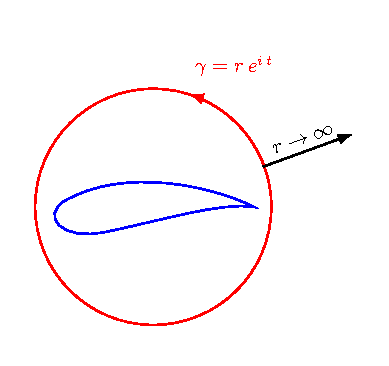
\includegraphics{papers/joukowski/images/04_komplexe_analysis/geschlossenes_linienintegral.pdf}
	\caption{
		Aufgrund der holomorphen Eigenschaft der Funktion kann das Linienintegral um den geschlossenen Kreisbogen $\gamma$,
		welches den Tragflügel komplett umschliesst, gemacht werden.
		Dabei kann der Radius beliebig gross gemacht werden,
		ohne dass sich das Resultat verändert.
		\label{joukowski:komplexe-analysis:fig:geschlossenes-linientintegral}}
\end{figure}


\subsubsection{Berechnung der Zirkulation $\Gamma$}
\begin{satz}
	\label{joukowski:komplexe-analysis:satz:zirkulation}
	$\Gamma = 2\pi i \cdot res(\overline{v(z)}, 0)$
\end{satz}

\begin{proof}
	\label{joukowski:komplexe-analysis:proof:zirkulation}
	Für die Auswertung von $\Gamma$ kann sehr ähnlich vorgegangen werden, wie bei der Berechnung von $\Lambda$ in Abschnitt~\ref{joukowski:komplexe-analysis:berechnung-von-lambda}.
	Auch da wählen wir den Kreis mit Zentrum bei $z_0 = 0$, mit Radius $r$ und die gleiche Parametrisierung von $z$.
	Für die Funtion $f(z) = \overline{v(z)}$ setzen wir die Reihenentwicklung aus der Gleichung~\eqref{joukowski:komplexe-analysis:laurent-reihe} ein.
	Somit wird aus dem Integral
	\[
	\Gamma
	=
	\displaystyle\int_{0}^{2\pi}
	\overline{v(r e^{i t})} \cdot i r e^{i t}
	dt
	\]
	der Ausdruck
	\[
	\begin{aligned}
		\Gamma
		&=
		\displaystyle\int_{0}^{2\pi}
		\biggl(v_\infty + \sum_{k=1}^{\infty} \frac{a_k}{r^k e^{k \cdot i t}}\biggr)
		i r e^{i t}
		dt \\
		\quad
		&=
		i\displaystyle\int_{0}^{2\pi}
		\biggl(v_\infty + \frac{a_1}{r e^{i t}} + \frac{a_2}{r^2 e^{2 i t}} + \frac{a_3}{r^3 e^{3 i t}} + \dots \biggr)
		r e^{i t}
		dt \\
		\quad
		&=
		i\displaystyle\int_{0}^{2\pi}
		\biggl(v_\infty r e^{i t} + a_1 + \frac{a_2}{r e^{i t}} + \frac{a_3}{r^2 e^{2 i t}} + \dots \biggr)
		dt.
	\end{aligned}
	\]
	Für die Auswertung dieses Integrals gibt es für die einzelnen Terme zwei verschiedene Auswertungen.
	Die Terme
	\[
	v_\infty r e^{i t}
	\quad
	\text{und}
	\quad
	\frac{a_k}{r^{k-1} e^{(k-1) \cdot i t}},
	\quad
	k \in [2, \infty)
	\]
	sind alle gleich wie bei der Berechnung von $\Lambda$ in der Gleichung~\eqref{joukowski:komplexe-analysis:integral-e-hoch-kit} periodisch,
	weshalb alle durch die Integration zu $0$ reduziert werden.
	
	Der einzige Term im Integral, welcher nicht verschwindet, ist $a_1$, der zu
	\[
	i\displaystyle\int_{0}^{2\pi}
	a_1
	dt
	=
	a_1 2\pi i
	\]
	ausgewertet wird.
	Somit gilt
	\begin{equation}
		\Gamma
		=
		a_1 2\pi i.
		\label{joukowski:komplexe-analysis:zirkulation-berechnet}
	\end{equation}
\end{proof}
Mit diesem Resultat können wir endlich die komplexe Kraft, welche auf das Flügelprofil wirkt ausrechnen.
Durch das Einsetzen von Gleichung~\eqref{joukowski:komplexe-analysis:zirkulation-berechnet}
in Satz~\ref{joukowski:komplexe-analysis:satz:kutta-joukowski}
erhalten wir den Term
\begin{equation}
	F'
	=
	-i \rho v_\infty \cdot a_1 2\pi i
	= \rho v_\infty a_1 2 \pi.
	\label{joukowski:komplexe-analysis:auftriebskraft-berechnet}
\end{equation}
Somit zeigt sich, dass nur ein Koeffizient der Laurent-Reihe, 
ausser die von uns vorgegebene Geschwindigkeit im Unendlichen $v_\infty$, 
einen Beitrag an der komplexen Kraft leistet, nämlich $a_1$.
Das heisst, dass dieser Koeffizient direkt bestimmt, 
ob eine reine Auftriebskraft resultiert, so wie wir das von unseren Voraussetzungen im Abschnitt~\ref{joukowski:sec:voraussetzungen} erwarten.
Oder ob zusätzlich noch einen Luftwiderstand sich bemerkbar macht.

Wir erwarten eine reine Auftriebskraft, was bedeutet, dass
\[
	F'
	=
	i F_y
	=
	\rho v_\infty a_1 2 \pi
\]
rein imaginär sein muss. Somit muss auch $a_1$ rein imaginär sein.

Im Abschnitt~\ref{joukowski:anwendungen} zeigen wir, wie der Koeffizient $a_1$ anhand von Beispielen von verschiedenen Flügelprofilen bestimmt werden kann.